
%(BEGIN_QUESTION)
% Copyright 2006, Tony R. Kuphaldt, released under the Creative Commons Attribution License (v 1.0)
% This means you may do almost anything with this work of mine, so long as you give me proper credit

Examine this cut-away illustration of a control valve packing assembly, located inside the bonnet of the valve:

$$\includegraphics[width=15.5cm]{i00879x01.eps}$$

Explain the purpose of each labeled component within the packing assembly.

\underbar{file i00879}
%(END_QUESTION)





%(BEGIN_ANSWER)

\noindent
{\bf Partial answer:}

\medskip
%\item{} Packing stud: a ``headless'' bolt, used to apply compressive force to the packing
%\item{} Packing nut: threads onto the stud, to apply compressive force to the packing
\item{} Packing flange: transfers force from nuts to the packing follower
\item{} Packing follower: transfers force from flange to the packing assembly
%\item{} Bushing(s): serve as guides for the valve stem, like linear bearings
%\item{} Anti-extrusion washer(s): help prevent packing material from ``extruding'' down the sides of the stem or the inside diameter of the bonnet
\item{} Lubrication port: lubricant is pumped in here
\item{} Lantern ring: allows even distribution of lubricant around the stem
%\item{} Packing ring(s): the actual sealing element against leakage
%\item{} Anti-extrusion ring(s): centers the packing ring(s) to help prevent extrusion
\item{} Packing box ring: provides a flat surface at the bottom of the assembly for the upper components to rest against
\end{itemize}

%(END_ANSWER)





%(BEGIN_NOTES)

\begin{itemize}
\item{} Packing stud: a ``headless'' bolt, used to apply compressive force to the packing
\item{} Packing nut: threads onto the stud, to apply compressive force to the packing
\item{} Packing flange: transfers force from nuts to the packing follower
\item{} Packing follower: transfers force from flange to the packing assembly
\item{} Bushing(s): serve as guides for the valve stem, like linear bearings
\item{} Anti-extrusion washer(s): help prevent packing material from ``extruding'' down the sides of the stem or the inside diameter of the bonnet
\item{} Lubrication port: lubricant is pumped in here
\item{} Lantern ring: allows even distribution of lubricant around the stem
\item{} Packing ring(s): the actual sealing element against leakage
\item{} Anti-extrusion ring(s): centers the packing ring(s) to help prevent extrusion
\item{} Packing box ring: provides a flat surface at the bottom of the assembly for the upper components to rest against
\end{itemize}


%INDEX% Final Control Elements, valve: valve packing assembly

%(END_NOTES)


